\documentclass[border=8pt]{standalone}
\usepackage{pgfplots}
\pgfplotsset{compat=1.18}
\begin{document}
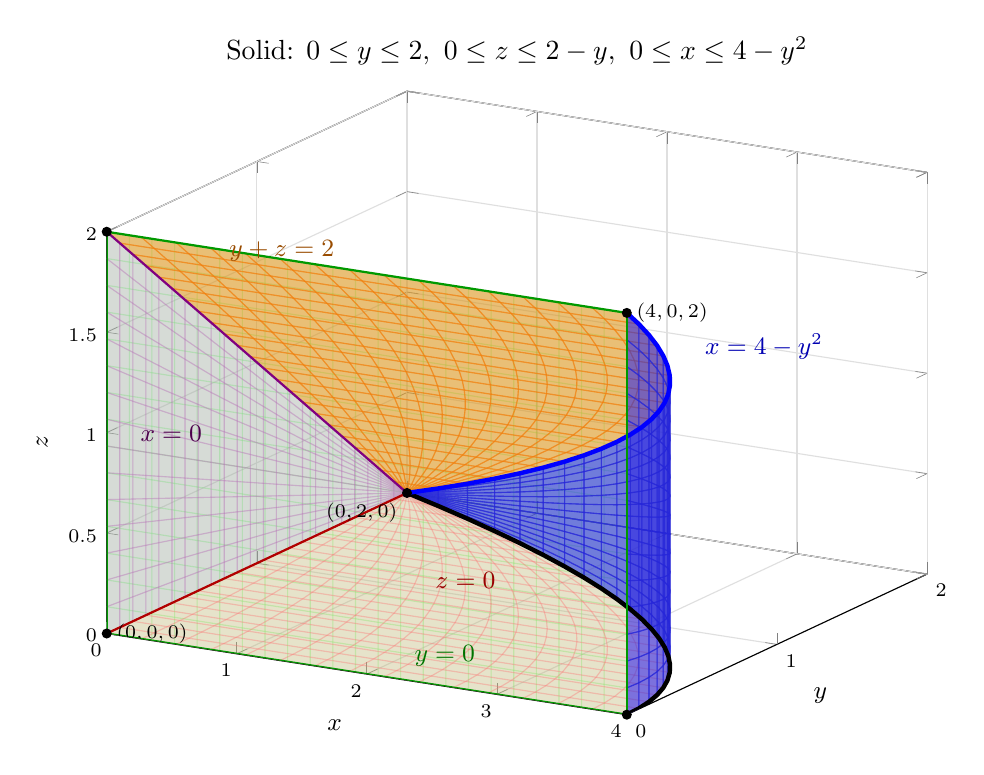
\begin{tikzpicture}
\begin{axis}[
    width=12cm, height=9.5cm,
    view={30}{22},
    xlabel={$x$}, ylabel={$y$}, zlabel={$z$},
    xmin=0, xmax=4, ymin=0, ymax=2, zmin=0, zmax=2,
    xtick={0,1,2,3,4}, ytick={0,1,2}, ztick={0,0.5,1,1.5,2},
    ticklabel style={font=\scriptsize},
    label style={font=\small},
    title={Solid: $0\le y\le 2,\ 0\le z\le 2-y,\ 0\le x\le 4-y^2$},
    grid=major, grid style={gray!25},
    axis background/.style={fill=white},
    samples=24, samples y=16,
]
\addplot3[surf, domain=0:1, domain y=0:1, color=green!55, opacity=0.22, shader=flat, draw=none]
({4*x}, {0}, {2*y});
\addplot3[surf, domain=0:2, domain y=0:1, color=red!55, opacity=0.20, shader=flat, draw=none]
({(4-x^2)*y}, {x}, {0});
\addplot3[surf, domain=0:2, domain y=0:1, color=violet!55, opacity=0.25, shader=flat, draw=none]
({0}, {x}, {(2-x)*y});
\addplot3[surf, domain=0:2, domain y=0:1, color=orange!80!brown, opacity=0.50, shader=flat, draw=none]
({(4-x^2)*y}, {x}, {2-x});
\addplot3[surf, domain=0:2, domain y=0:1, color=blue!70!gray, opacity=0.60, shader=flat, draw=none]
({4-x^2}, {x}, {(2-x)*y});

\addplot3[ultra thick, black, domain=0:2, samples y=1] ({4-x^2}, {x}, {0});
\addplot3[ultra thick, blue, domain=0:2, samples y=1] ({4-x^2}, {x}, {2-x});
\addplot3[thick, violet, domain=0:2, samples y=1] ({0}, {x}, {2-x});
\addplot3[thick, green!60!black, domain=0:4, samples y=1] ({x}, {0}, {0});
\addplot3[thick, green!60!black, domain=0:2, samples y=1] ({0}, {0}, {x});
\addplot3[thick, green!60!black, domain=0:4, samples y=1] ({x}, {0}, {2});
\addplot3[thick, green!60!black, domain=0:2, samples y=1] ({4}, {0}, {x});
\addplot3[thick, red!70!black, domain=0:2, samples y=1] ({0}, {x}, {0});

\addplot3[only marks, mark=*, mark size=1.6pt, black] coordinates {
 (0,0,0) (4,0,0) (0,0,2) (4,0,2) (0,2,0)
};
\node[font=\scriptsize, anchor=south east] at (axis cs:0,0,2)  {$(0,0,2)$};
\node[font=\scriptsize, anchor=north west] at (axis cs:4,0,0)  {$(4,0,0)$};
\node[font=\scriptsize, anchor=west]       at (axis cs:4,0,2)  {$(4,0,2)$};
\node[font=\scriptsize, anchor=north east] at (axis cs:0,2,0)  {$(0,2,0)$};
\node[font=\scriptsize, anchor=west]       at (axis cs:0,0,0)  {$(0,0,0)$};

\node[font=\small, blue!70!black, anchor=west]    at (axis cs:3.2,1.15,1.35) {$x=4-y^2$};
\node[font=\small, orange!60!black, anchor=south] at (axis cs:1.0,0.30,1.80) {$y+z=2$};
\node[font=\small, green!45!black,  anchor=south] at (axis cs:2.6,0,0.05)    {$y=0$};
\node[font=\small, red!60!black,    anchor=north] at (axis cs:1.2,1.35,0)    {$z=0$};
\node[font=\small, violet!60!black, anchor=east]  at (axis cs:0,0.70,0.75)   {$x=0$};
\end{axis}
\end{tikzpicture}
\end{document}